\chapter{Social Connectedness Index}

\resp{Bains, Arman Singh}

% \emph{
% Structure as\footnote{Remove this part from the report}:
% \begin{itemize}
% \item A short (max 1 page) explanation of the task, including references. Include mathematical concepts.
% \item Max 2 pages for the whole task (including figures)
% \item It is possible to use appendices for supplementary material, at the end of the report. Max 5 pages per task
% \end{itemize}
% A total of 3 pages + 5 supplementary pages per task
% }

% \section{A section...}
 
% Reference examples: book~\cite{barrat2008dynamical}, article~\cite{de2013mathematical}, website~\cite{weforumProtectingCritical}

\section{Introduction}

The goal of this project is to extract a network for each country from the Facebook Scaled Social Connectedness Index data \cite{facebook_sci}, which offers information on active Facebook users and their friendship networks. The \textit{Social Cennectedness Index} $SCI_{i,j}$ between two locations $i$ and $j$ is defined as:
$$SCI_{i,j}=\frac{FB\_Connections_{i,j}}{FB\_Users_i\cdot FB\_Users_j}$$
where $FB\_Users_i,FB\_Users_j$ are the number of Facebook users in locations $i,j$ and $FB\_Connections_{i,j}$ is the total number of Facebook friendship connections between individuals in the two locations. The \textit{Social Connectedness Index} available is actually rescaled so to have a maximum value of $1\cdot10^6$ and minimum of 1. \\
The main output consists of two files for each country, one concerning the nodes and other the edges of the networks (it's implied that such edges have weight equal to one, i.e. the networks are unweighted). An additional file has been produced, containing each edge's $SCI$, which was used to compute a few analytics, presented at the end of this chapter,

\section{Networks extraction}

The data downloaded \cite{facebook_sci} consisted in a TSV file built on the Database of Global Administrative Areas (GADM, version 2.8) and the European Nomenclature of Territorial Units for Statistics (NUTS 2016) areas. To ease the computation process, only the top 100 countries (encoded in \textit{gadm1}, \textit{gadm2} or \textit{nuts3} encoding) by total $SCI$ were considered (excluding USA). \\
The desired output consisted specifically in two files:
\begin{itemize}
    \item Edges: a file containing both nodes' IDs for each edge, alongside the name and ISO3 encoding for the country of the node from which the edge was originated
    \item Nodes: a file containing the ID and label of each node, alongside its latitude and longitude 
\end{itemize}

Whereas for \textit{gadm} encoded countries it was possible to convert the encoding to ISO3 just by string manipulation, \textit{nuts3} encoded nodes required the use of the \texttt{eurostat} \texttt{R} package, in particular of its function \texttt{get\_eurostat\_geospatial}, which allows one to store a shapefile that can be used to convert encodings. The encodings \texttt{EL} and \texttt{UK} were manually mapped to \texttt{GR} and \texttt{GB} respectively. \\
To add the coordinates to each node, for \textit{nuts3} encoded ares, the \texttt{get\_eurostat\_geospatial} function was again used, with a resolution of 60. In the other cases, it was possible to use a shapefile that was provided on the website alongside the rest of the data \cite{facebook_sci}. \\
After obtaining all the required data, for each country two separate CSV files were produced, with the characteristics described above. An extra file was produced for each country, in which in addition to the edges' information there is also their $SCI$.

A few graphs have been also proposed to gain a visual understanding of the networks. Figure \ref{fig:im} shows the relationship between mean degree and mean betweenness centrality, using as weight the $SCI$ of each edge. It's interesting to see that countries such as India and Germany seem to have very high mean degree but low mean betwenness, which is actually expected because they are subdivided in many interconnected administrative units, thus increasing their degree while lowering the average centrality. Figure \ref{fig:eig} instead shows instead the mean eigenvector centrality over the total $SCI$ per node. 

\begin{figure}[htbp]
    \centering
    \begin{minipage}[t]{0.48\linewidth}
        \centering
        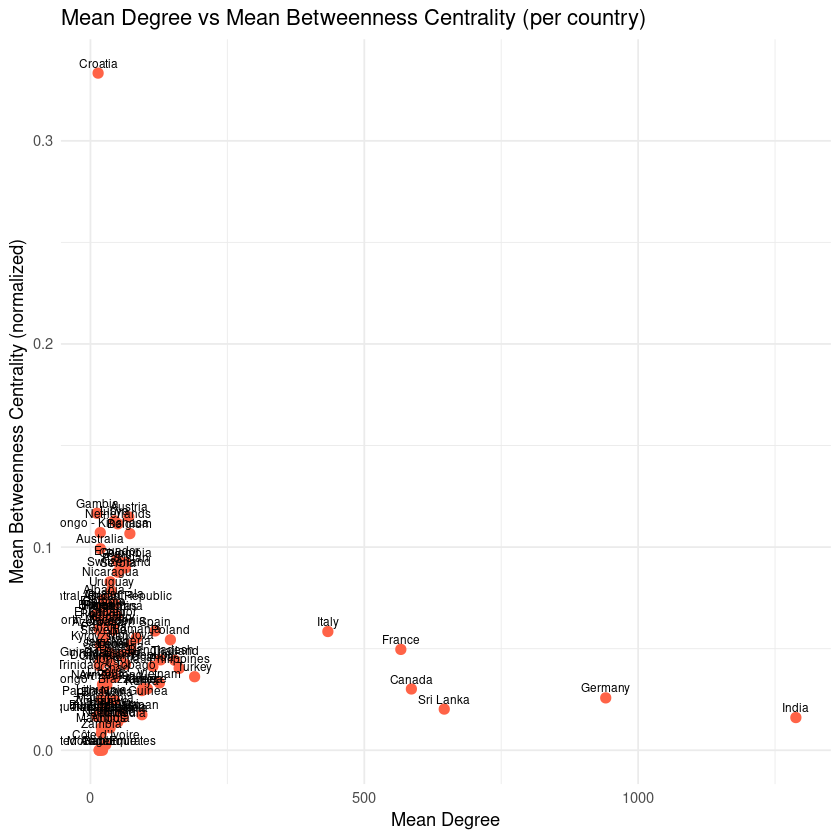
\includegraphics[width=\linewidth]{images/image.png}
        \caption{}
        \label{fig:im}
    \end{minipage}
    \hfill
    \begin{minipage}[t]{0.48\linewidth}
        \centering
        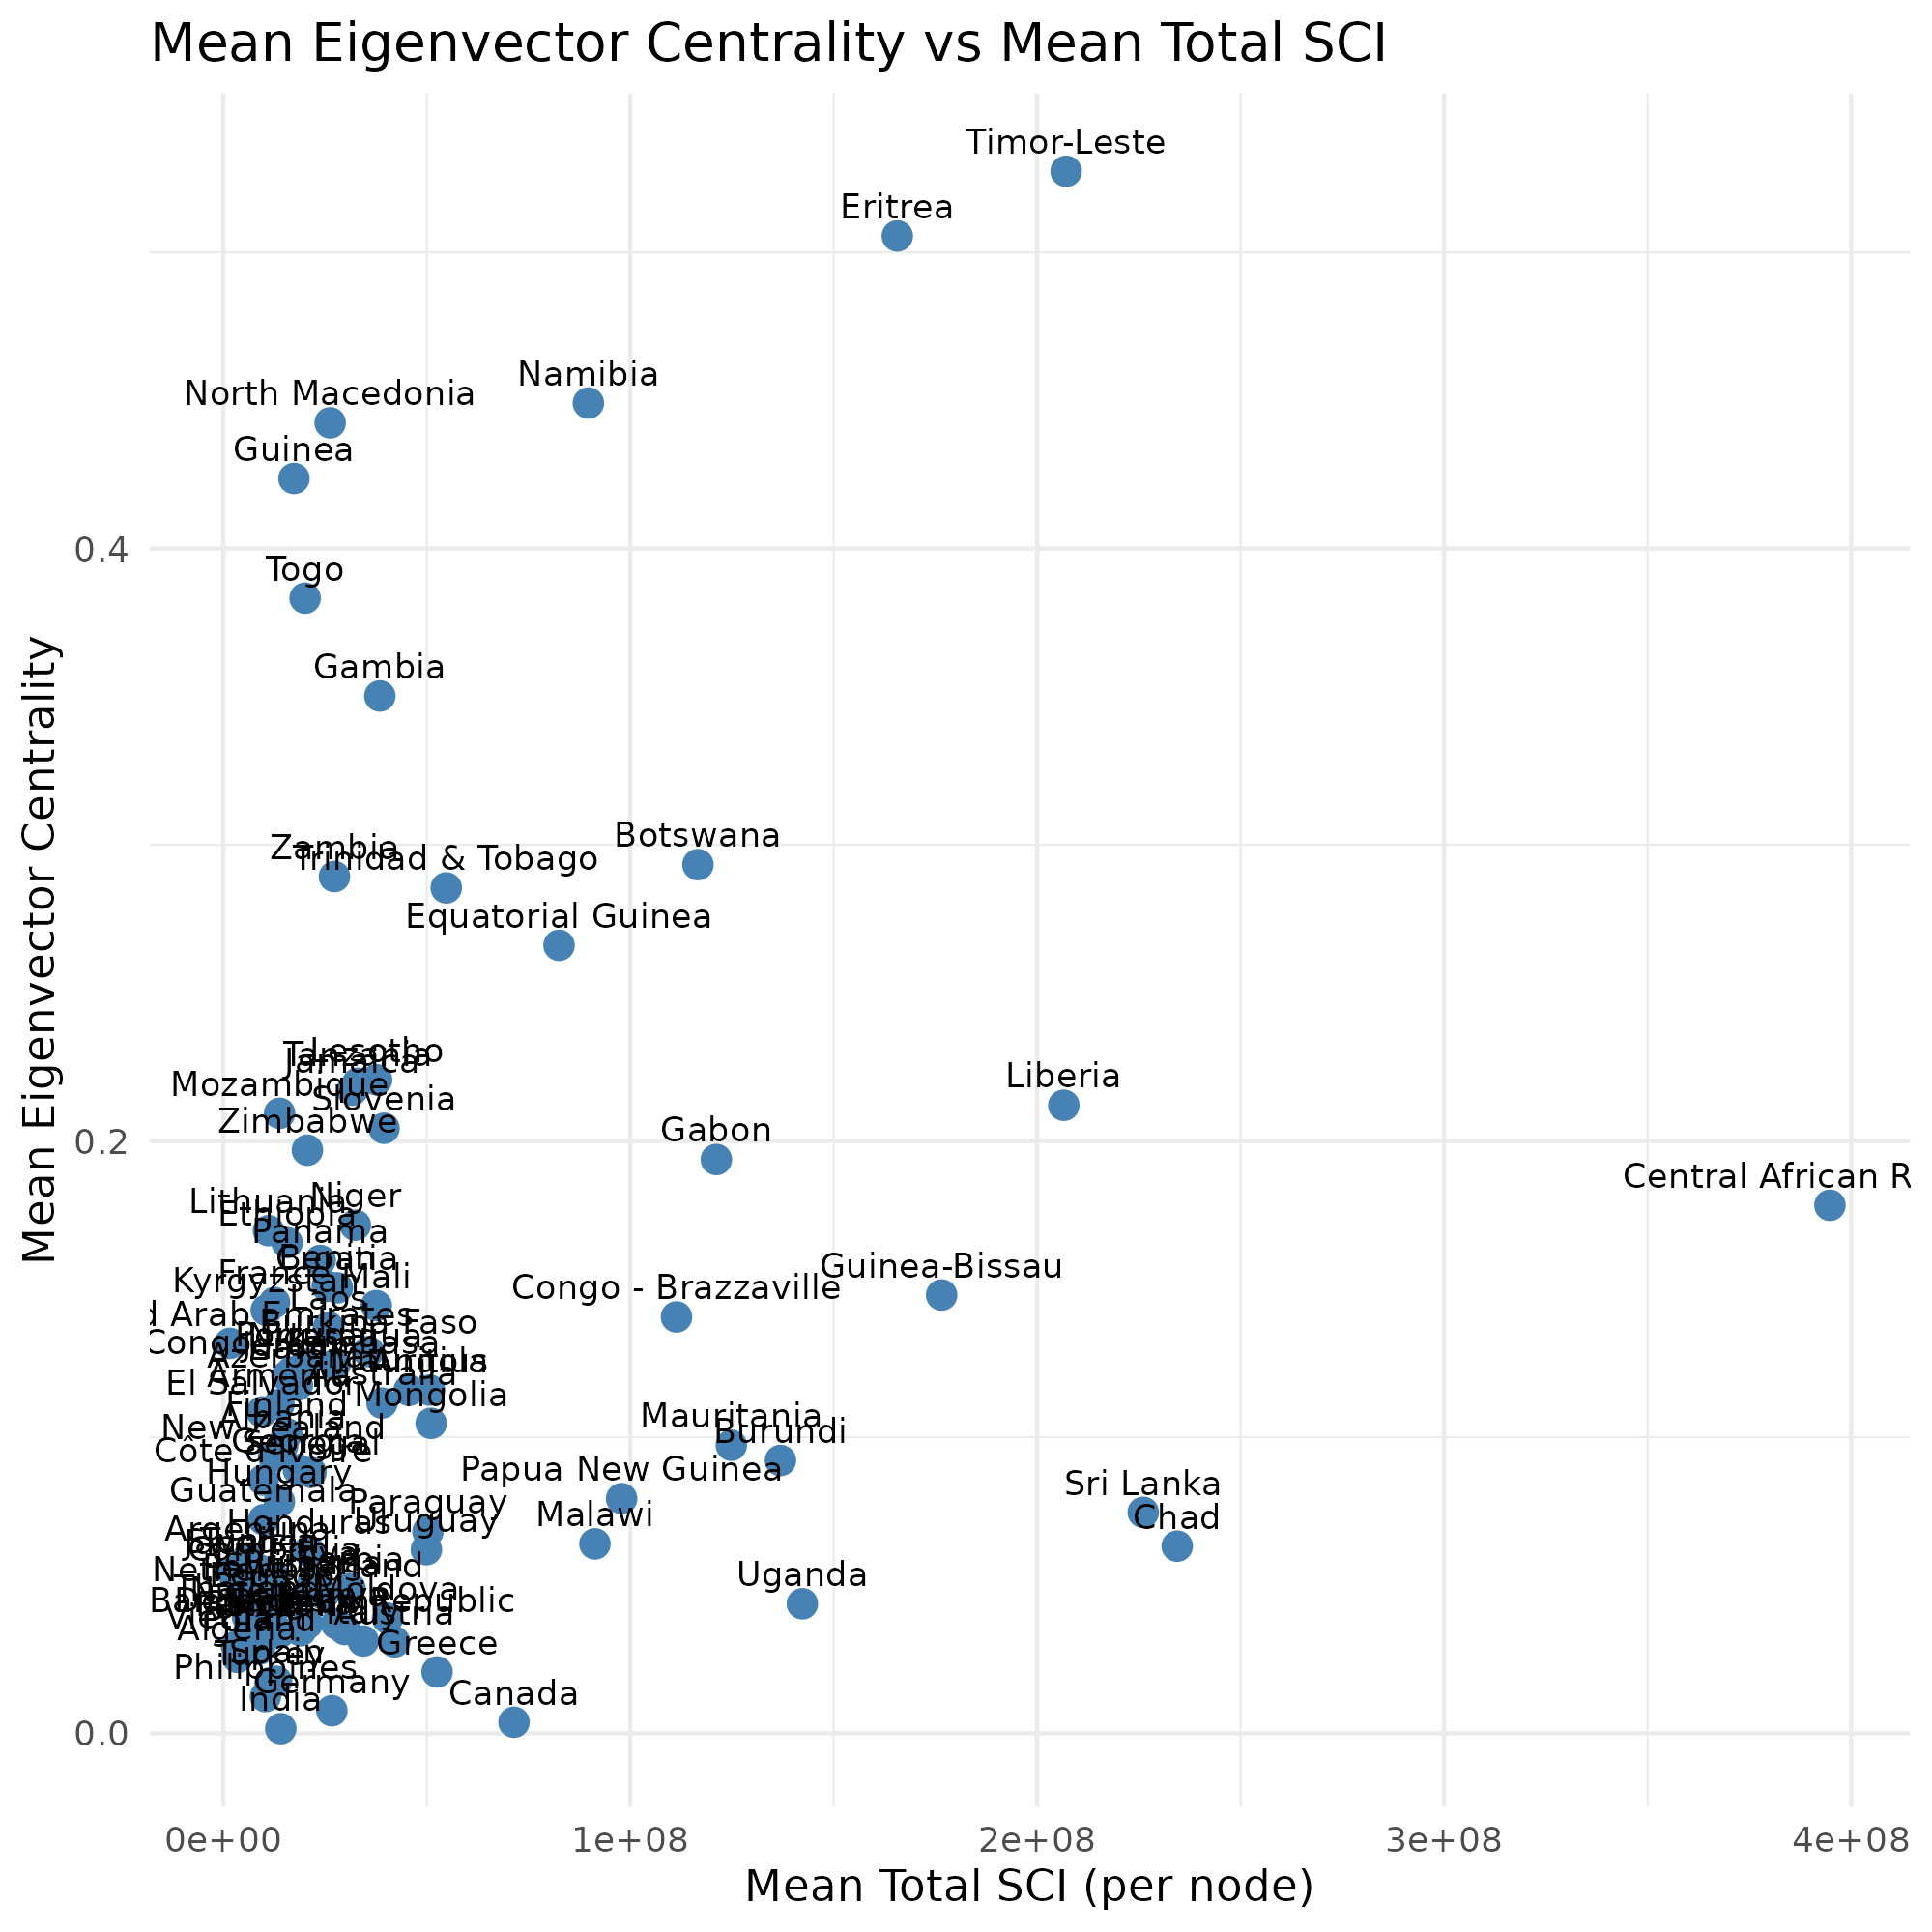
\includegraphics[width=\linewidth]{images/eig.png}
        \caption{}
        \label{fig:eig}
    \end{minipage}
    \label{fig:schelling1D}
\end{figure}


\newpage